\subsection{CUDA: acceleratore grafico}
\label{sec:cuda}
Con CUDA cambia il modello di esecuzione. Il pixel resta l'unità indipendente
(sezione~\ref{sec:parallelizzazione}), ma non viene più raggruppato in righe
distribuite fra poche unità di calcolo: ciascun pixel è affidato a uno dei
migliaia di thread della GPU.

L'hardware non esegue i thread singolarmente, ma li organizza in tre livelli. La
\emph{griglia} è l'insieme di tutti i \emph{blocchi}, ciascuno dei quali viene
assegnato per intero a uno Streaming Multiprocessor
(SM)~\cite{nvidia_ada_arch}. All'interno del blocco i thread sono numerati con la formula
$\texttt{id} = \texttt{threadIdx.x} + \texttt{threadIdx.y} \cdot
\texttt{blockDim.x}$, e l'SM li esegue in gruppi di $32$ id consecutivi ---
i \emph{warp}~\cite{nvidia_cuda_cc}. Ogni warp avanza con un unico program counter: i suoi $32$ thread
eseguono la stessa istruzione nello stesso ciclo secondo il modello SIMT
(Single Instruction, Multiple Threads). Il warp scheduler non conosce la
struttura 2D che si è dichiarata: vede solo id lineari e ne prende $32$ alla volta.

Questa linearizzazione è il punto critico per il problema in esame. Con
$\texttt{blockDim.x} = 32$, i thread $0$--$31$ hanno tutti
$\texttt{threadIdx.y} = 0$, cioè appartengono alla stessa riga del blocco; il
cambio di riga scatta solo all'id $32$, che è già nel warp successivo. Con
$\texttt{blockDim.x} = 16$, invece, il thread con $\texttt{id} = 16$ ha
$\texttt{threadIdx.x} = 0$, $\texttt{threadIdx.y} = 1$: il cambio di riga cade
a metà warp, e il warp $0$ finisce per contenere i pixel delle colonne $0$--$15$
della riga $0$ e delle colonne $0$--$15$ della riga $1$. In generale, per
$\texttt{blockDim.x}$ divisore di $32$, ogni warp copre $32/\texttt{blockDim.x}$
righe.

Quando un warp copre più righe si pongono due questioni distinte.
\begin{itemize}
    \item \textbf{Coalescenza.} La matrice è memorizzata in ordine row-major:
    pixel della stessa riga sono contigui in memoria, e $32$ scritture contigue
    possono essere servite in una sola transazione. Se il warp scrive su più
    righe gli indirizzi non sono più contigui e servono più transazioni, fino a
    $32$ volte il traffico per gli stessi dati.
    \item \textbf{Divergenza.} Le $32$ lane di un warp eseguono insieme, ma
    richiedono in generale un numero diverso di iterazioni: il warp termina solo
    quando termina la lane più lenta, e le lane già uscite consumano cicli con il
    risultato mascherato. Il costo del warp è quindi il massimo di $n_{i,j}$ sulle
    sue lane, invece della media, e la frazione di cicli sprecati è
    $1 - \overline{n}/\max n$. Un warp confinato in una riga non azzera la
    divergenza, perché una riga che attraversa il bordo contiene pixel interni ed
    esterni; un warp che riunisce righe diverse può però accostare situazioni
    ancora più eterogenee, per esempio pixel esterni in una riga e pixel di
    un'antenna nella riga successiva.
\end{itemize}
\vspace{3mm}
\begin{figure}[htbp]
    \centering
    \begin{subfigure}[t]{0.48\textwidth}
        \centering
        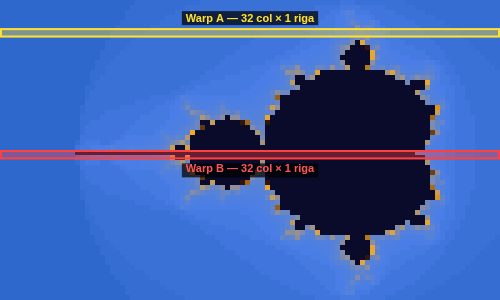
\includegraphics[width=\textwidth]{Immagini/warp_dim32}
        \caption{$\texttt{blockDim.x} = 32$: ogni warp occupa esattamente una riga.
        Il warp~A (giallo) cade in una zona esterna, dove tutti i pixel sfuggono in
        poche iterazioni; il warp~B (rosso) attraversa il bordo frattale, dove
        convivono pixel interni ed esterni con escape time molto diversi. Questa
        varianza dipende dalla geometria del problema, non dalla scelta del
        blocco.}
        \label{fig:warp-bdx32}
    \end{subfigure}
    \hfill
    \begin{subfigure}[t]{0.48\textwidth}
        \centering
        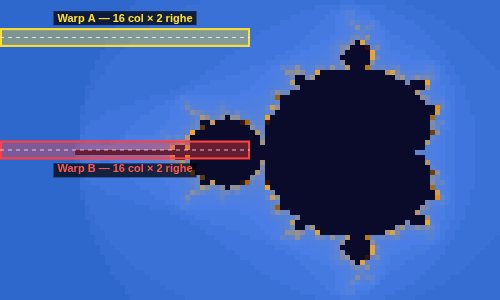
\includegraphics[width=\textwidth]{Immagini/warp_dim16}
        \caption{$\texttt{blockDim.x} = 16$: ogni warp copre due righe (la linea
        tratteggiata segna il confine). Il warp~A resta omogeneo, perché entrambe
        le righe cadono in zona esterna; nel warp~B le due righe possono
        campionare strutture diverse del bordo, e la varianza degli escape time
        può crescere rispetto al caso a riga singola.}
        \label{fig:warp-bdx16}
    \end{subfigure}
    \caption{Mappatura dei warp sulla griglia degli escape time al variare di
    $\texttt{blockDim.x}$; la risoluzione dell'immagine e l'estensione dei warp
    sono illustrative. In entrambe le figure sono evidenziati un warp in zona
    esterna (A, giallo) e uno sul bordo frattale (B, rosso). L'ipotesi illustrata è
    che riunire più righe in un warp possa aumentare la divergenza, oltre a
    spezzare la coalescenza; la sezione~\ref{sec:cuda-previsioni} ne quantifica
    l'effetto medio sull'intera immagine.}
    \label{fig:warp-divergenza}
\end{figure}
\vspace{5mm}
Come mostra la figura~\ref{fig:warp-divergenza}, la scelta
$\texttt{blockDim.x} = 32$, o un suo multiplo, garantisce che i $32$ id
consecutivi di un warp stiano sempre sulla stessa riga: le scritture restano
coalescenti, ed è esclusa la divergenza aggiuntiva dovuta all'accostamento di
righe diverse. $\texttt{blockDim.y}$ resta libero, perché determina quante righe
gestisce il blocco ma non la forma dei warp. Per questo la scelta
$\texttt{threadIdx.x} \to$ colonna, $\texttt{threadIdx.y} \to$ riga non è una
convenzione neutra. Si tratta tuttavia di un'ipotesi da verificare: un blocco
compatto riunisce pixel vicini in entrambe le direzioni, e in media potrebbe
produrre warp non meno omogenei di una riga. Le previsioni della
sezione~\ref{sec:cuda-previsioni} e le misure della
sezione~\ref{sec:cuda-risultati} ne quantificano l'effetto.

La varianza per pixel degli escape time è la stessa irregolarità discussa fin
dall'inizio del lavoro, che si manifesta come sbilanciamento del carico sulla CPU
e come divergenza dei warp sulla GPU.

L'aritmetica del kernel è identica a quella seriale, in doppia precisione, e il
build impone \texttt{-{}-fmad=false}, l'analogo per \texttt{nvcc} di
\texttt{-ffp-contract=off}: la contrazione in fused multiply-add cambierebbe
l'ultimo bit e quindi $\pm 1$ iterazione sui pixel di bordo, rendendo il checksum
incomparabile con la baseline. La L40S dispone inoltre di tensor core, progettati
per le moltiplicazioni fra matrici dense~\cite{nvidia_ada_arch}: il kernel,
scalare e per pixel, non ne fa uso per costruzione.

% ============================================================
\subsubsection{Design dello sweep}
\label{sec:cuda-sweep}
% ============================================================

La domanda progettuale è la stessa delle sezioni precedenti: \emph{come} mappare
il lavoro sulle unità di calcolo, non \emph{quanto}. Sulla GPU la variabile di
controllo non è il numero di core --- fisso per la scheda --- ma la
\emph{geometria del blocco}, ovvero la forma $B_x \times B_y$ con cui i thread vengono
organizzati, e che determina simultaneamente la struttura dei warp, la
coalescenza degli accessi in memoria e l'occupancy degli SM. Lo sweep si articola
in due esperimenti ortogonali, ciascuno con la propria domanda.

\paragraph{Sweep A --- geometria del blocco.}
Vengono fissati i parametri del problema ($1024^2$, $N_{\max}=1000$, come in
tutti gli altri sweep), e si fa variare la sola forma del blocco su nove
geometrie appartenenti a quattro gruppi distinti. L'esperimento risponde alla
domanda: qual è la mappatura thread$\to$pixel migliore, e perché?
La maggior parte delle geometrie ha lo stesso numero totale di thread
per blocco ($256$); ciò che varia è la loro distribuzione su righe e colonne,
che determina la struttura dei warp e quindi coalescenza e divergenza. Le due
eccezioni, $512{\times}1$ e $128{\times}1$, servono a isolare l'effetto
del numero di thread a geometria del warp fissa.

\begin{itemize}
    \item \textbf{Warp orizzontali puri} ($256{\times}1$, $512{\times}1$,
    $128{\times}1$): $\texttt{blockDim.x}$ multiplo di $32$, scritture
    coalescenti. Variano la taglia del blocco, e con essa potenzialmente
    l'occupancy, a coalescenza e divergenza fisse: è il gruppo di riferimento.
    \item \textbf{Quadrati 2D coalescenti} ($128{\times}2$, $64{\times}4$,
    $32{\times}8$): con \texttt{blockDim.x} multiplo di $32$, ogni warp prende 32 id consecutivi che
    stanno tutti sulla stessa riga. Quindi la coalescenza è intatta e la
    divergenza è la stessa dei warp orizzontali puri.
    La differenza rispetto al primo gruppo è solo \texttt{blockDim.y}:
    cambia quanti warp risiedono in un SM, e con essi potenzialmente l'occupancy.
    Isola l'effetto di avere più righe per
    blocco.
    \item \textbf{Coalescenza violata} ($16{\times}16$, $8{\times}32$):
    $\texttt{blockDim.x} < 32$, ogni warp ripiega su più righe, spezzando gli
    accessi in memoria in più transazioni. Questo gruppo mette in luce un aspetto interessante
    dello sweep: un quadrato compatto come $16{\times}16$
    raggruppa pixel più vicini fra loro e potrebbe avere divergenza
    \emph{inferiore} a quella dei warp orizzontali (campionando una regione più
    stretta del piano), ma a prezzo di coalescenza violata. Divergenza e
    coalescenza tirano in direzioni opposte: non esiste una scelta vincente a priori, e solo il tempo
    di esecuzione può stabilire quale effetto prevalga.
    \item \textbf{Warp verticale} ($1{\times}256$): la configurazione prevede $32$ pixel della stessa
    colonna, tali che gli indirizzi sono distanti $W \cdot 4$ byte l'uno dall'altro. Si tratta pertanto del caso
    peggiore per la coalescenza. La divergenza, però, è quasi identica
    a quella dei warp orizzontali: non c'è nessuna direzione privilegiata in cui il problema sia ``più omogeneo'' e,
    di conseguenza, la varianza di $n$ tra due pixel
    adiacenti in orizzontale è comparabile a quella tra due pixel adiacenti in
    verticale. Questo rende $256{\times}1$ contro $1{\times}256$ l'esperimento più pulito dello sweep: divergenza simile,
    coalescenza opposta. La differenza di tempo misurata è quindi imputabile
    principalmente alla penalità di coalescenza.
\end{itemize}

Vale la pena chiarire perché $1{\times}256$ non è l'analogo GPU della
decomposizione ciclica MPI. Nel ciclico MPI il rank $r$ riceveva righe sparse
per l'intera immagine, mescolando righe leggere e pesanti; l'analogo GPU sarebbe
un warp i cui $32$ pixel sono prelevati da righe distanti anziché adiacenti.
Quella configurazione avrebbe divergenza massima e accessi non coalescenti, e
sarebbe il caso peggiore per entrambe le leve; non è realizzabile con una forma
di blocco, ma il suo costo si può stimare dalla matrice degli escape time
(sezione~\ref{sec:cuda-previsioni}). La $1{\times}256$, invece, rompe la
coalescenza ma lascia pressoché intatta la divergenza, ed è per questo un
controllo utile.

Il risultato atteso dallo Sweep A è la classifica delle nove geometrie per
$T_{\min}$, insieme alla verifica di quanto le grandezze calcolabili dalla sola
matrice degli escape time (sezione~\ref{sec:cuda-previsioni}) ne anticipino
l'ordinamento: è l'analogo di $\lambda_p$, che sul lato CPU prevedeva lo speedup
(sezione~\ref{sec:serial-pred-lambdaP}).

\paragraph{Sweep B --- saturazione e trasferimento.}
Viene fissata la forma del blocco $256{\times}1$, riferimento a warp
orizzontali, e si fanno variare i valori dei parametri del problema. Sulla GPU
non è infatti il numero di core a variare, bensì il loro \emph{utilizzo}. La
scalabilità della GPU non è quindi una curva su $p$ come per OpenMP e MPI,
ma è una curva di \emph{saturazione}: al crescere della taglia del problema
cresce il numero di warp lanciati, e con essi l'occupazione degli SM, e le prestazioni in GFLOP/s, fino al
punto in cui aggiungere pixel non produce più guadagno proporzionale. Oltre
quella soglia la scheda è sfruttata appieno. Lo sweep si compone di due
esperimenti.

\textbf{B1 -- saturazione}: risoluzione $512^2 \to 1024^2 \to 2048^2 \to
4096^2$ a $N_{\max}=1000$ fisso.
Al crescere della risoluzione aumenta il
numero di warp lanciati e con essi l'occupazione degli SM: la curva di
throughput effettivo in GFLOP/s dovrebbe salire e appiattirsi verso il picco.
La domanda è \textit{da quale taglia} la scheda è sfruttata appieno, e quale
fattore la penalizza sotto quella soglia: overhead di lancio del kernel,
trasferimento incomprimibile o SM non saturi.

\textbf{B2 -- trasferimento}: $N_{\max} \in \{500, 1000, 5000\}$ a risoluzione
$2048^2$ fissa.
A pixel fissi i byte da copiare sono costanti, mentre il
calcolo cresce con $N_{\max}$: ci si attende che la frazione
$\texttt{transfer\_time}/T$ cali, mostrando l'ammortamento del costo di copia,
i cui contributi sono descritti nella sezione~\ref{sec:cuda-metriche}, al
crescere del lavoro. È il termine ``alla Amdahl'' del percorso
host$\leftrightarrow$device, e la curva B2 lo quantifica.

Ogni punto di B lancia il seriale e la GPU sullo stesso nodo nella stessa
esecuzione, così $S = T(1)/T_{\text{gpu}}$ è same-hardware per costruzione: un
core CPU contro una GPU, con la baseline seriale rigenerata a ogni confronto. Il
punto a $1024^2$ e $N_{\max}=1000$ ripete la configurazione $256{\times}1$ dello
Sweep~A con lo stesso numero di ripetizioni, e fa quindi da controllo fra i due
job.

% ============================================================
\subsubsection{Metriche specifiche}
\label{sec:cuda-metriche}
% ============================================================

Sulla GPU il numero di core è fissato dalla scheda e non è una variabile
controllabile: al crescere del problema cresce la loro occupazione, non il loro
numero. Il parametro $p$ è quindi degenere, e con esso efficienza e metrica di
Karp--Flatt, che presuppongono un numero variabile di unità di calcolo. Lo
speedup è definito come $S = T_1/T_{\text{gpu}}$, dove $T_1$ è il tempo della
baseline seriale su un core della CPU dello stesso nodo: è il confronto fra due
implementazioni dello stesso problema, non fra configurazioni a $p$ variabile.

Tre grandezze sono proprie di questo paradigma.

La \textbf{divergenza} è misurata tramite un proxy deterministico calcolato
dalla matrice degli escape time: per ogni gruppo di $32$ pixel contigui secondo
la mappatura del kernel, si calcola la varianza dei valori $n_{i,j}$; la media
di queste varianze su tutti i gruppi è il proxy. Poiché l'unico branch del
kernel è il ciclo di escape, la divergenza dipende soltanto dagli escape time dei
pixel riuniti nel warp, ed è quindi interamente calcolabile dalla matrice. Questo approccio è preferibile alla misura
strumentata con un profiler per tre ragioni: è deterministico e privo di rumore,
non richiede permessi sui performance counter (spesso non disponibili sui
cluster), e non perturba i tempi di esecuzione.

L'\textbf{occupancy} è teorica e si ottiene dall'API runtime. In linea di
principio il suo valore dipende dal numero di registri che il kernel impiega per
thread, riportato da \texttt{-Xptxas -v}: il kernel mantiene attive più
variabili in doppia precisione ($z_{\text{real}}$, $z_{\text{imag}}$, i
rispettivi quadrati, $c_{\text{real}}$ e $c_{\text{imag}}$), e registri
insufficienti limiterebbero i warp che possono risiedere contemporaneamente su un
SM. Un'occupancy elevata non implica tuttavia prestazioni migliori: serve a
mascherare le latenze di memoria, mentre il kernel è limitato dal calcolo, con
fino a $8\,N_{\max}$ FLOP per ogni scrittura da $4$ byte. La leva attesa come
primaria è quindi la divergenza.

Il \textbf{tempo di trasferimento} device$\to$host è misurato con CUDA event
attorno alla copia della matrice risultante ($4$ byte per pixel). Non esiste
traffico host$\to$device: gli input del kernel sono scalari passati come
argomenti al lancio, senza alcuna \texttt{cudaMemcpy}.
Poiché il costo di copia è fisso in byte mentre il calcolo cresce con
$N_{\max}$, la grandezza di interesse è la frazione $\texttt{transfer\_time}/T$, che è attesa calare
all'aumentare di $N_{\max}$: lo Sweep~B2 quantifica questo ammortamento.

\paragraph{Che cosa comprende il tempo di trasferimento.}
La copia della matrice dalla GPU alla memoria del processo non è un'unica
operazione: il tempo misurato somma tre contributi,
\[
    T_{\text{transfer}} = T_{\text{PCIe}} + T_{\text{socket}} + T_{\text{host}}.
\]
\begin{itemize}
    \item $T_{\text{PCIe}}$ è il trasferimento sul bus della scheda, un
    collegamento PCIe~4.0~x16 con una banda nominale di circa $31{,}5$~GB/s per
    direzione;
    \item $T_{\text{socket}}$ è l'eventuale attraversamento
    dell'interconnessione fra i due socket del nodo, nullo quando il processo
    gira sul socket a cui è collegata la GPU;
    \item $T_{\text{host}}$ è la copia in memoria host: la matrice risiede in
    memoria ordinaria, che la GPU non può scrivere direttamente, per cui il
    driver trasferisce i dati in un buffer intermedio e li copia poi nella
    destinazione.
\end{itemize}

Il termine centrale dipende da una scelta che non è sotto il controllo del job.
Il nodo è dual-socket (sezione~\ref{sec:ambiente}), e ciascuna delle otto GPU è
collegata a uno dei due socket; in assenza di richieste esplicite, SLURM assegna
la GPU e il core del processo in base alla disponibilità del momento. Da un job
all'altro il processo può quindi trovarsi sullo stesso socket della GPU, il caso
locale, oppure sull'altro, il caso cross-NUMA (figura~\ref{fig:numa-topology}).
Poiché \texttt{nvidia-smi} non riporta l'affinità NUMA della scheda, il job dello
Sweep~B la ricava da \texttt{sysfs} e registra nel log sia il socket del
processo sia i core locali alla GPU
(\repofile{mandelbrot/job_sbatch/mandel_cuda_scaling.sh}). Ogni valore di
\texttt{transfer\_time} viene così letto rispetto al posizionamento effettivo del
proprio job, e non rispetto a uno presunto.
\vspace{2,5mm}
\begin{figure}[htbp]
    \centering
    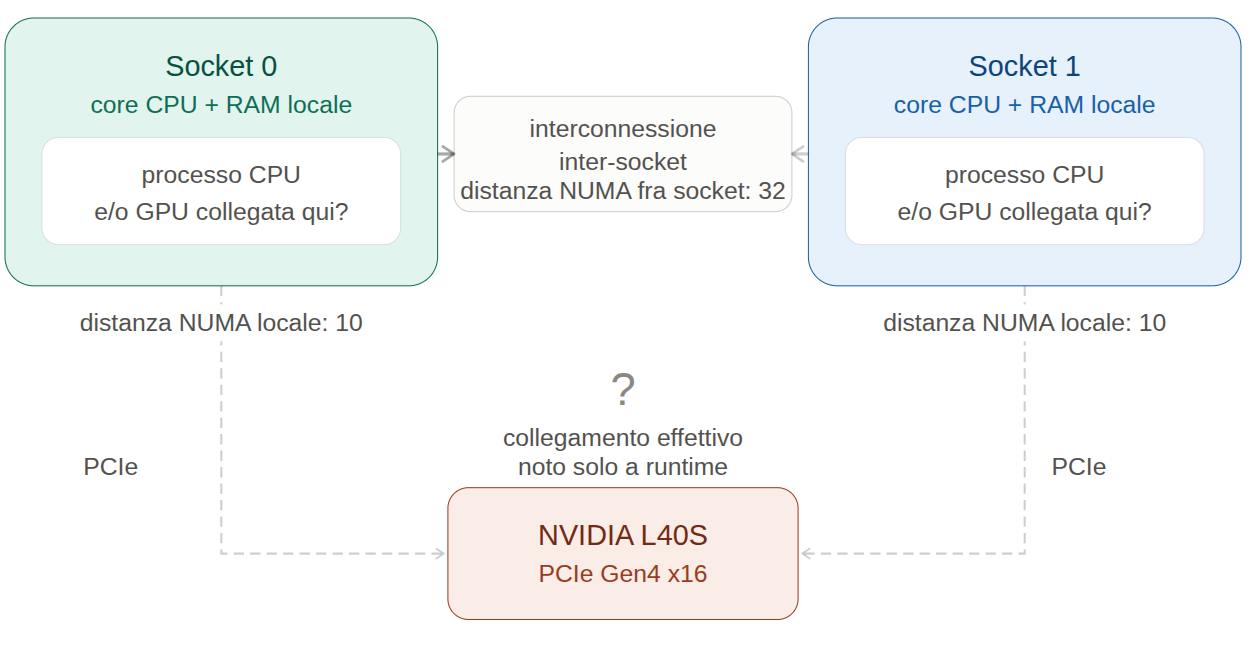
\includegraphics[width=0.8\textwidth]{Immagini/numa_topology}
    \caption{Topologia NUMA di \texttt{gnode01}. Ciascun socket dispone dei
    propri core e della propria memoria locale; i due socket sono collegati da
    un'interconnessione, per la quale il firmware dichiara una distanza NUMA di
    $32$ contro $10$ dell'accesso locale, un valore relativo e non una misura di
    latenza. La GPU è collegata tramite PCIe a uno dei due socket, e il processo
    può essere eseguito sullo stesso socket o sull'altro: nel secondo caso la
    copia della matrice attraversa anche l'interconnessione.}
    \label{fig:numa-topology}
\end{figure}

% ============================================================
\subsubsection{Frammenti di codice rilevanti}
\label{sec:cuda-codice}
% ============================================================

Nei due paradigmi precedenti il kernel seriale restava riconoscibile: OpenMP vi
anteponeva una direttiva, MPI lo racchiudeva in un protocollo di messaggi. Con
CUDA scompaiono invece i due cicli annidati sui pixel: ogni thread esegue una
sola volta il corpo del ciclo e deve ricavare autonomamente il pixel di propria
competenza. La ricorrenza di escape è identica a quella seriale e non viene
riportata; il codice completo è in \repofile{mandelbrot/src/mandelbrot_cuda.cu}.

\begin{verbatim}
__global__ void mandelbrot_kernel(int* escape_counts, int width, int rows,
                                  Viewport view, double dx, double dy,
                                  int max_iter) {
    const int col = blockIdx.x * blockDim.x + threadIdx.x;
    const int row = blockIdx.y * blockDim.y + threadIdx.y;
    if (col >= width || row >= rows) return;     // lanes beyond the image

    // c_real, c_imag: centre of pixel (row, col), as in the serial kernel
    escape_counts[row * width + col] = escape_time(c_real, c_imag, max_iter);
}
\end{verbatim}

Le variabili \texttt{col} e \texttt{row} realizzano l'intera assegnazione del
lavoro. Ogni thread dispone di tre terne predefinite: \texttt{threadIdx}, la
posizione del thread all'interno del proprio blocco, con componenti comprese fra
$0$ e $\texttt{blockDim}-1$; \texttt{blockIdx}, la posizione del blocco
all'interno della griglia; \texttt{blockDim}, le dimensioni del blocco. Lungo
ciascun asse il prodotto $\texttt{blockIdx}\cdot\texttt{blockDim}$ è il numero di
thread contenuti nei blocchi che precedono quello corrente, e coincide quindi con
la coordinata del primo pixel del blocco; sommandovi \texttt{threadIdx} si ottiene
la coordinata globale del thread. \texttt{col} è pertanto l'indice di colonna del
pixel e \texttt{row} il suo indice di riga (\texttt{rows} coincide con l'altezza
dell'immagine quando la simmetria non è attiva): la coppia individua l'unica cella
della matrice degli escape time che il thread calcola e scrive. L'associazione
dell'asse $x$ alle colonne è la scelta motivata nella sezione~\ref{sec:cuda}. Come
l'indice di riga globale dei rank MPI (sezione~\ref{sec:mpi-codice}), il compito
non viene comunicato al thread ma ricavato dalla sua posizione; a differenza di
MPI, l'unità assegnata non è una riga ma un singolo pixel.

La guardia successiva è necessaria perché la griglia è dimensionata per eccesso
(frammento seguente): quando le dimensioni dell'immagine non sono multiple di
quelle del blocco, i blocchi dell'ultima riga o colonna della griglia si
estendono oltre l'immagine, e i thread corrispondenti devono terminare senza
scrivere. Si osservi infine che nessuna istruzione del kernel dipende dalla forma
del blocco: le nove geometrie dello Sweep~A eseguono lo stesso codice e
differiscono soltanto per l'insieme di pixel che condividono un warp.

\begin{verbatim}
static const dim3 block = block_shape_from_env();       // MANDEL_BLOCK=BXxBY
static const double occupancy = launch_occupancy(block);
const dim3 grid((width + block.x - 1) / block.x,          // ceiling division
                (computed_rows + block.y - 1) / block.y);
mandelbrot_kernel<<<grid, block>>>(d_escape_counts, width, computed_rows, ...);
\end{verbatim}

La forma del blocco è letta a esecuzione dalla variabile d'ambiente
\texttt{MANDEL\_BLOCK}, analogamente a quanto avviene con la variabile
\texttt{OMP\_SCHEDULE} per OpenMP e con la variabile \texttt{MPI\_DECOMP} per
MPI: un solo eseguibile copre così tutte le geometrie dello sweep. Forma del blocco e occupancy, che dipende soltanto da essa, sono
determinate una volta per processo (\texttt{static}); la griglia è invece
ricalcolata a ogni chiamata, poiché dipende dalla risoluzione, che lo Sweep~B fa
variare.

Il frammento più rilevante per l'analisi non appartiene al kernel, ma al codice
condiviso delle metriche (\repofile{mandelbrot/src/metrics.cpp}), che calcola
divergenza e spreco sulla matrice degli escape time. Per
ogni blocco della griglia, di indici \texttt{bx} e \texttt{by}, i thread vengono
raggruppati in warp di $32$ id consecutivi e ciascun id viene ricondotto al
proprio pixel:

\begin{verbatim}
for (long long start = 0; start < threads_per_block; start += warp_size) {
    lane.clear();                            // lanes of one warp
    const long long end = std::min(start + warp_size, threads_per_block);
    for (long long id = start; id < end; ++id) {
        const int col = bx * block_x + static_cast<int>(id % block_x);
        const int row = by * block_y + static_cast<int>(id / block_x);
        if (col < width && row < height)
            lane.push_back(img.data[row * width + col]);
    }
    // accumulate var(lane) and 1 - mean(lane) / max(lane)
}
\end{verbatim}

Le espressioni di \texttt{col} e \texttt{row} sono quelle del kernel, con la
posizione del thread nel blocco ricavata dall'id lineare invertendo la formula
della sezione~\ref{sec:cuda}: $\texttt{threadIdx.x} = \texttt{id} \bmod
\texttt{blockDim.x}$ e $\texttt{threadIdx.y} = \lfloor \texttt{id} /
\texttt{blockDim.x} \rfloor$. Il raggruppamento riproduce quindi esattamente
quello operato dal warp scheduler, ed è per questo che divergenza e spreco sono
previsioni disponibili prima dell'esecuzione del kernel. Le lane che cadono oltre
l'immagine sono escluse, affinché entrambe le grandezze misurino la variabilità
indotta dal frattale e non gli effetti di bordo della suddivisione in blocchi.
Coerentemente con il contratto delle metriche, il calcolo risiede nel driver
condiviso e non nel kernel.

Due ulteriori accorgimenti allineano la regione misurata al contratto comune agli
altri paradigmi (allocazione inclusa, I/O escluso):

\begin{verbatim}
const ContextInit g_context_init;   // ctor: cudaFree(nullptr) -> context

cudaEventRecord(before_copy);       // queued behind the kernel, same stream
cudaMemcpy(img.data.data(), d_escape_counts, bytes, cudaMemcpyDeviceToHost);
cudaEventRecord(after_copy);        // elapsed(before, after) = pure D2H
\end{verbatim}

Il primo riguarda il contesto CUDA, la cui creazione, eseguita alla prima
chiamata all'API, richiede centinaia di millisecondi: l'oggetto statico
\texttt{g\_context\_init} lo crea prima dell'avvio del cronometro, così che il
costo non ricada sulla prima ripetizione. Il secondo riguarda il tempo di
trasferimento: i due event sono accodati sullo stesso stream del kernel, che
esegue le operazioni in ordine, quindi \texttt{before\_copy} viene raggiunto solo
al termine del kernel e l'intervallo misurato comprende la sola copia
device$\to$host.

Le grandezze proprie della GPU raggiungono il CSV attraverso accessori dichiarati
nell'header comune (\texttt{kernel\_occupancy()},
\texttt{kernel\_transfer\_seconds()} e le dimensioni del blocco), che i kernel
CPU definiscono nulli: il medesimo driver produce così lo stesso schema di record
per tutti i paradigmi.

% ============================================================
\subsubsection{Previsioni dalla matrice degli escape time}
\label{sec:cuda-previsioni}
% ============================================================

% Fonte: data/block_geometry.csv (analysis/block_geometry.py su
% figure_nmax1000.raw, matrice nuda 1024^2, N_max=1000, W = 259655490);
% divergenza e spreco coincidono con cuda_log_notes_34335.txt. Registri per
% thread dal log di build (-Xptxas -v).

Come per le decomposizioni CPU (sezione~\ref{sec:serial-pred-lambdaP}), il costo
delle geometrie del blocco può essere stimato prima di eseguire il kernel. La
forma del blocco determina quali pixel condividono un warp, e questo
raggruppamento è riproducibile sulla matrice degli escape time del baseline con
l'attraversamento della sezione~\ref{sec:cuda-codice}. Divergenza e spreco sono
calcolati anche dal binario CUDA durante lo sweep; cicli e costo dei blocchi sono
stati ricavati successivamente dalla stessa matrice, con
\repofile{mandelbrot/analysis/block_geometry.py}. In entrambi i casi le grandezze
dipendono dai soli dati seriali, ed è in questo senso che costituiscono
previsioni a priori.

Per ciascuna geometria si considerano quattro grandezze:
\begin{itemize}
    \item la \textbf{divergenza} e lo \textbf{spreco medio}, definiti
    rispettivamente nelle sezioni~\ref{sec:cuda-metriche} e~\ref{sec:cuda};
    \item i \textbf{cicli relativi}: poiché un warp termina solo quando termina
    la sua lane più lenta, i cicli eseguiti con una geometria sono
    $\sum_{\text{warp}} \ell \cdot \max n_{i,j}$, con $\ell$ numero di lane del
    warp; il loro rapporto con quelli della $256{\times}1$ è il tempo relativo
    previsto nell'ipotesi che il tempo sia proporzionale ai cicli;
    \item il \textbf{CoV del costo dei blocchi}, coefficiente di variazione dei
    cicli eseguiti per blocco, che descrive la granularità con cui il lavoro è
    suddiviso.
\end{itemize}
Non si riporta invece il rapporto fra costo massimo e costo medio dei blocchi,
che sarebbe l'analogo di $\lambda_p$: non appena un blocco cade interamente
all'interno dell'insieme, il suo costo è $N_{\max}$ per lane, e il rapporto si
riduce a $N_{\max}$ diviso i cicli medi per pixel ($1000/286{,}4 = 3{,}49$ per
tutte le geometrie orizzontali), senza alcuna informazione sulla forma del
blocco.
\vspace{2,5mm}
\begin{table}[htbp]
    \centering
    \begin{tabular}{lrrrrr}
        \hline
        Blocco & divergenza & spreco medio & cicli relativi & CoV blocchi & occ. \\
        \hline
        $128{\times}1$ & $10\,215$ & $11{,}24\%$ & $1{,}000$ & $1{,}41$ & $1{,}00$ \\
        $256{\times}1$ & $10\,215$ & $11{,}24\%$ & $1{,}000$ & $1{,}34$ & $1{,}00$ \\
        $512{\times}1$ & $10\,215$ & $11{,}24\%$ & $1{,}000$ & $1{,}25$ & $1{,}00$ \\
        $128{\times}2$ & $10\,215$ & $11{,}24\%$ & $1{,}000$ & $1{,}41$ & $1{,}00$ \\
        $64{\times}4$  & $10\,215$ & $11{,}24\%$ & $1{,}000$ & $1{,}51$ & $1{,}00$ \\
        $32{\times}8$  & $10\,215$ & $11{,}24\%$ & $1{,}000$ & $1{,}54$ & $1{,}00$ \\
        \hline
        $16{\times}16$ & $5\,932$  & $7{,}82\%$  & $0{,}947$ & $1{,}59$ & $1{,}00$ \\
        $8{\times}32$  & $3\,689$  & $6{,}23\%$  & $0{,}928$ & $1{,}59$ & $1{,}00$ \\
        \hline
        $1{\times}256$ & $9\,550$  & $11{,}75\%$ & $0{,}998$ & $1{,}33$ & $1{,}00$ \\
        \hline
        sparso         & $131\,050$ & $66{,}31\%$ & $2{,}501$ & --- & --- \\
        \hline
    \end{tabular}
    \caption{Previsioni per le geometrie dello Sweep~A, calcolate dalla sola
    matrice degli escape time del baseline ($1024^2$, $N_{\max}=1000$, kernel
    \emph{bare}) e, per l'occupancy, dall'API runtime. Le righe sono raggruppate
    per partizione in warp: orizzontale, compatta, verticale e sparsa. I cicli
    sono relativi alla $256{\times}1$. Il raggruppamento sparso non è realizzabile
    con una forma di blocco.}
    \label{tab:cuda-previsioni}
\end{table}

\paragraph{Quattro partizioni in nove geometrie.}
Il proxy vale $10\,215$ per tutte le sei geometrie con $\texttt{blockDim.x}$
multiplo di $32$. In questo caso, all'interno di ogni warp,
$\texttt{id} \bmod \texttt{blockDim.x}$ assume $32$ valori consecutivi e
$\lfloor \texttt{id}/\texttt{blockDim.x} \rfloor$ resta costante: il warp è
formato da $32$ pixel contigui della stessa riga, e ogni riga risulta suddivisa
in segmenti di $32$ pixel indipendentemente da $\texttt{blockDim.y}$. La
partizione in warp è quindi la stessa, e con essa divergenza, spreco e cicli; le
sei forme differiscono soltanto per la granularità dei blocchi, come mostra la
colonna del CoV. Le nove geometrie realizzano pertanto quattro partizioni
distinte. Le due compatte, $8{\times}32$ e $16{\times}16$, riuniscono pixel più
vicini nel piano e riducono i cicli del $7{,}2\%$ e del $5{,}3\%$; quella
verticale, $1{\times}256$, è quasi equivalente all'orizzontale ($-0{,}24\%$). Fra
le forme realizzabili il modello attribuisce dunque alla geometria del blocco un
peso di pochi punti percentuali. In media, inoltre, la matrice non conferma che
riunire righe diverse aumenti la divergenza: le partizioni compatte la riducono. I
casi locali di forte eterogeneità illustrati nella
figura~\ref{fig:warp-divergenza} restano possibili, ma pesano poco sulla media
dell'intera immagine.

\paragraph{Occupancy.}
L'occupancy prevista vale $1{,}00$ per tutte le geometrie. Il kernel impiega $22$
registri per thread, secondo il log di compilazione. Per la compute
capability~$8.9$ un SM dispone di $64$\,K registri e ospita al più $1\,536$
thread residenti, cioè $48$ warp da $32$ thread~\cite{nvidia_cuda_cc}: i
registri basterebbero per circa $90$ warp, ben oltre il limite, per cui il
vincolo effettivo è il numero di thread e non la disponibilità di registri. Tutte le geometrie usano inoltre
blocchi da $128$, $256$ o $512$ thread, divisori dei $1\,536$ thread di un SM,
che viene così riempito senza posti residui. L'occupancy non può dunque
distinguere le geometrie, e l'ipotesi della sezione~\ref{sec:cuda-metriche},
secondo cui il numero di variabili del kernel FP64 ne avrebbe limitato il valore,
è smentita già prima dell'esecuzione.

\paragraph{Il raggruppamento sparso.}
Nella forma calcolata, il pixel $p$ della matrice linearizzata è assegnato al
warp $p \bmod 32\,768$: ogni warp contiene $32$ pixel della stessa colonna, a
$32$ righe di distanza l'uno dall'altro, e campiona quindi l'intera altezza
dell'immagine. Il proxy vale $131\,050$, $12{,}8$ volte quello della partizione
orizzontale, lo spreco medio sale al $66\%$ e i cicli a $2{,}5$ volte: è il caso
peggiore anticipato nella sezione~\ref{sec:cuda-sweep}.

% ============================================================
\subsubsection{Analisi dei risultati}
\label{sec:cuda-risultati}
% ============================================================

% Dati Sweep A: job 34334 (--repeat 10) e 34335 (--repeat 30) su gnode01,
% partizione only-one-gpu, L40S, entrambi COMPLETED 0:0. Fonti: run_34334.csv,
% run_34335.csv e le note cuda_log_notes_*.txt, che conservano warp_div_scat,
% warp_wasted e i registri/thread: figure assenti dal CSV e presenti solo nel
% log di job, che non e' versionato.
%
% Previsioni: sec:cuda-previsioni (data/block_geometry.csv).
%
% Dati Sweep B: job 34424 su gnode01, partizione only-one-gpu, L40S diversa da
% quella dello Sweep A (UUID GPU-a554e585...), 30 ripetizioni GPU e 3 seriali.
% Fonti: run_34424.csv e cuda_log_notes_34424.txt, che conserva il
% posizionamento NUMA (GPU sul nodo 0, processo sul core 42 del socket 1).
% Regressioni (tempo di copia sui byte; T = c + tau*W nel B2) calcolate dai
% valori del CSV.

\paragraph{Sweep A -- geometria del blocco.}
La tabella~\ref{tab:cuda-blocks} riporta le nove geometrie, misurate in due
campagne distinte; tutte producono lo stesso checksum della baseline seriale.
Fra la più veloce ($1{\times}256$, $5{,}631$~ms) e la più lenta ($64{\times}4$,
$6{,}091$~ms) il divario è dell'$8{,}2\%$: su questo kernel la geometria del
blocco è una leva di second'ordine. I paragrafi seguenti verificano che il
divario sia sistematico, lo confrontano con le previsioni della
sezione~\ref{sec:cuda-previsioni} (occupancy e cicli) ed esaminano infine i due
effetti che la tabella delle previsioni non contiene: coalescenza e granularità
dei blocchi.
\vspace{2,5mm}
\begin{table}[htbp]
    \centering
    \caption{Sweep~A: tempi misurati per le nove geometrie del blocco ($1024^2$,
        $N_{\max}=1000$, kernel \emph{bare}), nello stesso ordine della
        tabella~\ref{tab:cuda-previsioni}. Le due colonne di tempo corrispondono ai
        job $34334$ ($10$ ripetizioni) e $34335$ ($30$ ripetizioni), entrambi su
        \texttt{gnode01}, partizione \texttt{only-one-gpu}. Il tempo relativo è
        riferito alla $256{\times}1$ nella campagna a $30$ ripetizioni e va letto
        contro i cicli relativi previsti; lo speedup è riferito alla baseline
        seriale del job $34335$, $T(1) = 0{,}720255$~s.}
    \label{tab:cuda-blocks}
    \begin{tabular}{lrrrr}
        \hline
        Blocco & $T_{\min}^{(10)}$ [ms] & $T_{\min}^{(30)}$ [ms] & $T/T_{256\times1}$ & $S$ \\
        \hline
        $128{\times}1$ & $5{,}802$ & $5{,}690$ & $0{,}985$ & $126{,}6$ \\
        $256{\times}1$ & $5{,}814$ & $5{,}776$ & $1{,}000$ & $124{,}7$ \\
        $512{\times}1$ & $6{,}057$ & $5{,}988$ & $1{,}037$ & $120{,}3$ \\
        $128{\times}2$ & $5{,}984$ & $5{,}957$ & $1{,}031$ & $120{,}9$ \\
        $64{\times}4$  & $6{,}244$ & $6{,}091$ & $1{,}055$ & $118{,}2$ \\
        $32{\times}8$  & $6{,}116$ & $6{,}086$ & $1{,}054$ & $118{,}3$ \\
        \hline
        $16{\times}16$ & $5{,}877$ & $5{,}860$ & $1{,}015$ & $122{,}9$ \\
        $8{\times}32$  & $5{,}865$ & $5{,}752$ & $0{,}996$ & $125{,}2$ \\
        \hline
        $1{\times}256$ & $5{,}623$ & $\mathbf{5{,}631}$ & $0{,}975$ & $127{,}9$ \\
        \hline
    \end{tabular}
\end{table}

\paragraph{Riproducibilità della classifica.}
Sei delle nove geometrie hanno $\texttt{blockDim.x}$ multiplo di $32$ e, come mostrato
nella sezione~\ref{sec:cuda-previsioni}, suddividono l'immagine negli stessi warp: divergenza, spreco e
occupancy coincidono, e nessuna di queste grandezze le distingue. Nella campagna
a $10$ ripetizioni i loro tempi minimi coprivano tuttavia un intervallo del
$7{,}6\%$, più del doppio del vantaggio della $1{\times}256$ sulla $256{\times}1$
($3{,}4\%$). Con una dispersione di tale ampiezza fra configurazioni equivalenti
rispetto ai predittori, non era possibile stabilire se la classifica fosse
riproducibile. La campagna a $30$ ripetizioni risolve la questione: l'ordinamento
si ripete con un solo scambio, fra la terza e la quarta posizione ($8{\times}32$
e $256{\times}1$, distanti lo $0{,}4\%$); nessun tempo minimo varia di più del
$2{,}5\%$ fra le due campagne, e quello della $1{\times}256$ varia dello
$0{,}14\%$. Le differenze sono quindi sistematiche e richiedono una spiegazione.

La stessa campagna conferma la scelta di $T_{\min}$ come statistica di
riferimento. Per la $8{\times}32$ si ha $T_{\text{mean}} = 11{,}21$~ms a fronte
di $T_{\text{median}} = 6{,}05$~ms: la mediana, allineata a quella delle altre
geometrie, esclude un rallentamento dell'intera serie, mentre lo scarto della
media corrisponde a un ritardo cumulato di circa $155$~ms sulle $30$ ripetizioni,
compatibile con una singola esecuzione disturbata da un evento esterno. Il minimo
non ne risente.

\paragraph{Occupancy.}
L'occupancy rilevata vale $1{,}00$ per tutte le geometrie, come previsto nella
sezione~\ref{sec:cuda-previsioni}, e non può quindi spiegare le differenze di tempo.

\paragraph{Cicli previsti e tempi misurati.}
La tabella~\ref{tab:cuda-previsioni} attribuisce alle partizioni compatte una
riduzione dei cicli del $7{,}2\%$ ($8{\times}32$) e del $5{,}3\%$ ($16{\times}16$)
rispetto alla $256{\times}1$. Se il tempo fosse determinato dai cicli dei warp, le
due geometrie dovrebbero risultare più veloci in misura analoga. La
tabella~\ref{tab:cuda-blocks} non lo conferma: la $8{\times}32$ guadagna lo
$0{,}4\%$ e la $16{\times}16$ è più lenta dell'$1{,}5\%$.

La previsione non è per questo errata: i cicli sono un calcolo esatto sulla
matrice e quantificano correttamente il lavoro mascherato. Ciò che la misura
smentisce è
l'ipotesi, formulata nella sezione~\ref{sec:cuda-metriche}, che tale lavoro sia la
leva primaria del tempo di esecuzione: nell'intervallo esplorato, riduzioni dei
cicli dei warp fino al $7\%$ non producono guadagni apprezzabili. Individuare la
componente che domina il tempo richiederebbe una misura strumentata, non
disponibile su questo cluster (si veda oltre).

\paragraph{Coalescenza.}
Il confronto fra $256{\times}1$ e $1{\times}256$ era stato progettato per isolare
la penalità di coalescenza. Le due geometrie hanno divergenza simile ($10\,215$ e
$9\,550$) e, secondo la tabella~\ref{tab:cuda-previsioni}, un numero di cicli dei warp che
differisce dello $0{,}24\%$; la prima scrive però $32$ indirizzi contigui per
warp, la seconda $32$ indirizzi distanti $4\,096$ byte l'uno dall'altro. In
presenza di una penalità di coalescenza la $1{\times}256$ risulterebbe più lenta;
la misura la indica invece più veloce del $2{,}5\%$ ($3{,}4\%$ nella campagna a
$10$ ripetizioni).

L'assenza di penalità si spiega confrontando il traffico di memoria con la banda
disponibile. Il kernel scrive $4$~MiB per lancio in $5{,}63$~ms, pari a circa
$0{,}74$~GB/s, a fronte degli $864$~GB/s di banda di memoria della
scheda~\cite{nvidia_ada_arch}. Anche
ammettendo che la perdita di coalescenza moltiplichi il traffico per il fattore
massimo di $32$ (sezione~\ref{sec:cuda}), si otterrebbero circa $24$~GB/s, meno
del $3\%$ della banda. In nessuna delle due configurazioni il canale di memoria si
avvicina alla saturazione, e il numero di transazioni non incide quindi sul tempo.
Il risultato costituisce la verifica sperimentale di quanto la
sezione~\ref{sec:cuda-metriche} aveva argomentato per via teorica: il kernel è
limitato dal calcolo e non dalla banda.

\paragraph{Granularità dei blocchi.}
Fra le tre geometrie orizzontali pure, che condividono partizione in warp,
divergenza, spreco e occupancy, il tempo cresce con la dimensione del blocco in
entrambe le campagne: $128{\times}1$ ($8\,192$ blocchi da $4$ warp,
$5{,}690$~ms), $256{\times}1$ ($4\,096$ blocchi da $8$ warp, $5{,}776$~ms),
$512{\times}1$ ($2\,048$ blocchi da $16$ warp, $5{,}988$~ms). Poiché l'unica
grandezza che varia è il numero di blocchi, la differenza del $5\%$ va attribuita
alla granularità con cui il lavoro viene distribuito sui $142$ SM del
chip~\cite{nvidia_ada_arch}.
L'interpretazione coerente con i dati è che blocchi più piccoli consentano di
ripartire il carico fra gli SM in modo più uniforme, avvicinando il completamento
dell'ultimo SM a quello medio. Ciò vale nonostante i blocchi più piccoli abbiano,
singolarmente, un costo più variabile (CoV $1{,}41$ contro $1{,}25$): è il loro
numero maggiore per SM a mediare il carico. Si tratta dello stesso meccanismo osservato con il
chunk in OpenMP (sezione~\ref{sec:openmp-risultati}), dove a $32$ thread
\texttt{dynamic,1} risultava cinque volte più veloce di \texttt{dynamic,64}.
L'effetto è qui molto più contenuto perché anche la geometria più grossolana, con
$2\,048$ blocchi, resta di gran lunga più fine dei $16$ chunk di
\texttt{dynamic,64}.

La granularità non spiega tuttavia tutte le differenze osservate. Le geometrie
$128{\times}2$, $64{\times}4$ e $32{\times}8$ hanno la stessa partizione in warp e
lo stesso numero di thread per blocco della $256{\times}1$, dunque la stessa
granularità, eppure risultano più lente dal $3$ al $5{,}5\%$. Questo scarto e il
primato della $1{\times}256$ sono i due risultati dello sweep che nessuna delle
grandezze previste spiega, e vengono pertanto riportati come questioni aperte.

\paragraph{Assenza di una misura strumentata.}
In entrambi i job la misura di conferma con \texttt{ncu} è fallita con l'errore
\texttt{ERR\_NVGPUCTRPERM}: l'accesso ai performance counter della GPU è riservato
agli amministratori, secondo l'impostazione predefinita di NVIDIA per i sistemi
multiutente. L'esecuzione è proseguita, poiché la chiamata era protetta in
previsione di questo caso. Divergenza e occupancy restano quindi prive di una
conferma strumentata, e il proxy deterministico è l'unica misura disponibile della
divergenza, come previsto nella sezione~\ref{sec:cuda-metriche}. Per la stessa
ragione le due questioni aperte dello Sweep~A non possono essere indagate su
questo cluster.

\paragraph{Il raggruppamento ciclico sulla GPU.}
Il raggruppamento sparso, analogo GPU della decomposizione ciclica, richiederebbe
secondo la tabella~\ref{tab:cuda-previsioni} $2{,}5$ volte i cicli della
partizione orizzontale, con uno spreco medio del $66\%$. Su MPI la stessa idea
--- mescolare righe leggere e pesanti --- era il rimedio allo sbilanciamento di
carico (sezione~\ref{sec:mpi-risultati}); sotto SIMT produce l'effetto opposto,
perché riunisce nello stesso warp pixel con escape time eterogenei e moltiplica i
cicli mascherati. La causa è unica, la varianza per-pixel degli escape time, ma i
rimedi sono contrari: su memoria distribuita conviene mescolare il carico fra le
unità di calcolo, sotto SIMT conviene raggruppare pixel simili.

La portata di questa conclusione va però delimitata. Il raggruppamento sparso non
è realizzabile con una forma di blocco, perché richiederebbe una permutazione
degli indici nel kernel, e non è stato misurato. Lo Sweep~A ha inoltre mostrato
che, nell'intervallo esplorato, il tempo è poco sensibile ai cicli dei warp: una
riduzione del $7{,}2\%$ si è tradotta in un guadagno dello $0{,}4\%$. Che un
aumento dei cicli di $2{,}5$ volte produca un rallentamento comparabile resta
dunque una previsione del modello, non un risultato sperimentale.

\paragraph{Throughput e confronto con la CPU.}
% Fonti: FP32 90,5 TFLOPS dall'appendice sulla L40 (stesso chip AD102 della
% L40S) di nvidia_ada_arch; rapporto FP32:FP64 = 64 dalla tabella 30 di
% nvidia_cuda_cc per la compute capability 8.9 e dalla nota sui core FP64 di
% nvidia_ada_arch.
La geometria più veloce raggiunge $369$~GFLOP/s. La documentazione NVIDIA
riporta per la L40, basata sullo stesso chip AD102 della L40S, un throughput FP32
di picco di $90{,}5$~TFLOPS, e un rapporto di $64$ fra throughput FP32 e
FP64~\cite{nvidia_ada_arch,nvidia_cuda_cc}: il picco in doppia precisione è
quindi di circa $1\,414$~GFLOP/s. Il kernel se ne colloca al $26\%$, mentre rispetto
al picco FP32 si colloca allo $0{,}4\%$. Le due percentuali descrivono aspetti
distinti: la prima indica quanto siano sfruttate le unità di calcolo in doppia
precisione, la seconda quanto sia sfruttata la scheda nel suo complesso. Il divario dipende
dalla doppia precisione, imposta dal contratto di riproducibilità, e motiva un
eventuale esperimento in singola precisione; i picchi sono valori nominali, non
misurati sul cluster.

Lo speedup rispetto alla baseline seriale misurata nello stesso job è $S = 128$.
Il confronto più significativo è però con il miglior risultato CPU della campagna,
il master--worker MPI con $32$ unità di calcolo ($23{,}156$~ms,
sezione~\ref{sec:mpi-risultati}): una sola GPU è $4{,}11$ volte più veloce di $32$
core. Il trasferimento device$\to$host richiede fra $0{,}214$ e $0{,}228$~ms,
circa il $3{,}8\%$ di $T_{\min}$ per la geometria più veloce, e non varia
apprezzabilmente fra le geometrie, come atteso dato che la quantità di dati
copiati è la stessa.

\paragraph{Sweep B -- saturazione e trasferimento.}
La tabella~\ref{tab:cuda-scaling} riporta la curva di saturazione (B1) e la
frazione di trasferimento al variare di $N_{\max}$ (B2). Tutte le sei
configurazioni riproducono il checksum della rispettiva baseline seriale,
misurata nello stesso job.
\vspace{2,5mm}
\begin{table}[htbp]
    \centering
    \caption{Sweep B: saturazione (B1, $N_{\max}=1000$) e frazione di trasferimento
        (B2, risoluzione $2048^2$), con blocco $256{\times}1$; job $34424$ su
        \texttt{gnode01}, $30$ ripetizioni per la GPU e $3$ per il seriale. $\Pi$ è
        il throughput effettivo in GFLOP/s e $S$ lo speedup rispetto al seriale
        della stessa configurazione; copia$/T$ è la frazione
        $\texttt{transfer\_time}/T_{\min}$; la banda è quella effettiva della copia
        device$\to$host, cioè i byte copiati divisi per \texttt{transfer\_time}.
        Il punto $2048^2$, $N_{\max}=1000$ è comune ai due esperimenti.}
    \label{tab:cuda-scaling}
    \small
    \begin{tabular}{llrrrrr}
        \hline
        Sweep & problema & $T_{\min}$ [ms] & $\Pi$ [GFLOP/s] & $S$ & copia$/T$ [\%] & banda [GB/s] \\
        \hline
        B1 & $512^2$   & $2{,}565$  & $202{,}5$ & $70{,}4$  & $3{,}49$ & $11{,}7$ \\
        B1 & $1024^2$  & $5{,}735$  & $362{,}2$ & $125{,}8$ & $3{,}91$ & $18{,}7$ \\
        B1 & $2048^2$  & $19{,}131$ & $434{,}3$ & $150{,}6$ & $4{,}57$ & $19{,}2$ \\
        B1 & $4096^2$  & $75{,}705$ & $439{,}0$ & $152{,}2$ & $3{,}74$ & $23{,}7$ \\
        \hline
        B2 & $N_{\max}{=}500$  & $10{,}446$ & $406{,}9$ & $140{,}0$ & $7{,}08$ & $22{,}7$ \\
        B2 & $N_{\max}{=}1000$ & $19{,}131$ & $434{,}3$ & $150{,}6$ & $4{,}57$ & $19{,}2$ \\
        B2 & $N_{\max}{=}5000$ & $87{,}474$ & $465{,}2$ & $162{,}5$ & $0{,}84$ & $23{,}0$ \\
        \hline
    \end{tabular}
\end{table}

\paragraph{Controllo fra i due job.}
Il punto a $1024^2$ e $N_{\max}=1000$ ripete la configurazione $256{\times}1$
dello Sweep~A: $5{,}735$~ms contro $5{,}776$~ms, uno scarto dello $0{,}7\%$,
entro la variabilità osservata fra job distinti. Il confronto vale più di quanto
sembri, perché i log mostrano che i due job hanno usato due schede L40S
fisicamente diverse: la differenza fra le due schede non supera il rumore di
misura, e le due campagne sono direttamente confrontabili. Anche la baseline
seriale coincide entro lo $0{,}2\%$.

\paragraph{Saturazione (B1).}
Il throughput effettivo cresce con la risoluzione e poi si stabilizza
(figura~\ref{fig:cuda-saturation}): $202$,
$362$, $434$ e $439$~GFLOP/s da $512^2$ a $4096^2$. Fra le ultime due taglie il
guadagno è dell'$1\%$ a fronte di un lavoro quadruplicato: la scheda è satura da
circa $2048^2$, cioè da circa quattro milioni di pixel. Poiché il costo medio per
pixel è identico in tutte le taglie ($248$ iterazioni), la differenza dipende
soltanto da quanto efficacemente la GPU viene sfruttata. Lo speedup rispetto a un
core segue lo stesso andamento, da $70$ a $152$, mentre il seriale resta fermo a
circa $2{,}88$~GFLOP/s.
\begin{figure}[htbp]
    \centering
    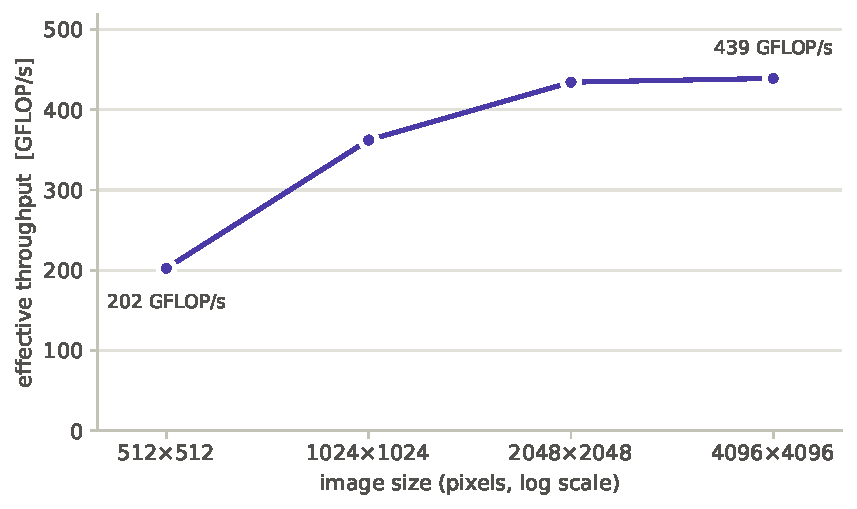
\includegraphics[width=0.85\textwidth]{Immagini/grafici/cuda_saturation}
    \caption{Throughput effettivo della GPU in funzione della dimensione
    dell'immagine (Sweep~B1: blocco $256{\times}1$, $N_{\max}=1000$, job $34424$).
    Il throughput si stabilizza da $2048^2$; il seriale, a circa
    $2{,}88$~GFLOP/s, non è rappresentabile sulla stessa scala.}
    \label{fig:cuda-saturation}
\end{figure}

Dei tre fattori attesi, il trasferimento si può escludere: pesa fra il $3{,}5$ e
il $4{,}6\%$ del tempo a ogni taglia, e non può spiegare un throughput dimezzato.
Anche un costo fisso di lancio spiega poco. I tempi delle due taglie maggiori
crescono in proporzione ai pixel, e la loro retta attribuisce al costo
indipendente dalla taglia circa $0{,}3$~ms; a $512^2$, però, il tempo misurato
supera quella previsione del $77\%$, e a $1024^2$ del $15\%$. La penalità delle
taglie piccole è quindi compatibile con il terzo fattore, il sottoutilizzo della
scheda: con pochi pixel non ci sono abbastanza warp da tenere occupati tutti gli
SM. Senza performance counter non è possibile verificarlo direttamente. Il proxy
di divergenza diminuisce con la risoluzione, da $18\,012$ a $3\,154$, perché pixel
adiacenti diventano più simili; lo Sweep~A ha però mostrato che i cicli sprecati
incidono poco sul tempo, e non possono spiegare la saturazione.

Rispetto al seriale la GPU conviene già alla taglia minima ($S = 70$). Il
confronto con la CPU parallela è disponibile solo a $1024^2$, dove una GPU resta
$4{,}04$ volte più veloce del master--worker MPI su $32$ unità, in accordo con lo
Sweep~A.

\paragraph{Trasferimento (B2) e posizionamento NUMA.}
A risoluzione fissa i byte copiati sono costanti ($16$~MiB), mentre il lavoro
cresce con $N_{\max}$: la frazione del tempo spesa nella copia scende dal
$7{,}1\%$ a $N_{\max}=500$ allo $0{,}8\%$ a $N_{\max}=5000$, come atteso. Un
modello lineare sui tre punti, $T = c + \tau\,\mathcal{W}$, riproduce i tempi
entro $0{,}06$~ms e separa un costo di circa $1{,}5$~ms indipendente da
$N_{\max}$ (copia, allocazione e lancio a questa taglia) da un throughput
marginale di $473$~GFLOP/s, il valore verso cui tende quello effettivo al
crescere del lavoro.

Il log del job documenta il posizionamento: la GPU assegnata ha come core locali
$0$--$31$, cioè il nodo NUMA $0$, mentre il processo è stato eseguito sul core
$42$, sul socket $1$. È il caso cross-NUMA descritto nella
sezione~\ref{sec:cuda-metriche}: ogni copia attraversa anche l'interconnessione
fra i socket. La banda effettiva cresce con la dimensione della copia
(figura~\ref{fig:cuda-copy}), da
$11{,}7$~GB/s per $1$~MiB a $23{,}7$~GB/s per $64$~MiB. Interpolando il tempo di
copia in funzione dei byte si ottengono una banda di circa $24$~GB/s e un costo
fisso di circa $0{,}07$~ms per copia, che penalizza le copie piccole. La banda
asintotica è quindi circa il $77\%$ dei $31{,}5$~GB/s nominali del PCIe~4.0~x16.
A parità di byte la banda oscilla fra $19{,}2$ e $23{,}0$~GB/s nelle tre
esecuzioni a $2048^2$: la singola copia è soggetta a una variabilità non
trascurabile.
\begin{figure}[htbp]
    \centering
    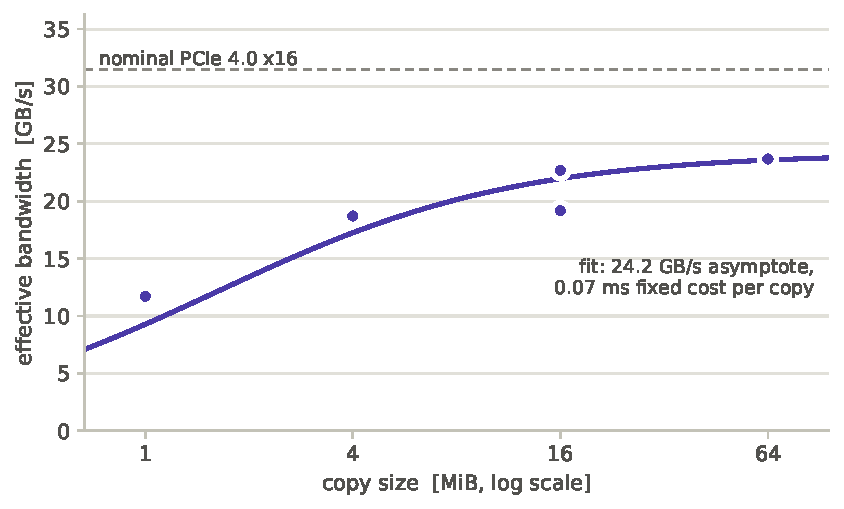
\includegraphics[width=0.85\textwidth]{Immagini/grafici/cuda_copy_bandwidth}
    \caption{Banda effettiva della copia device$\to$host in funzione della
    dimensione della copia, per le sei configurazioni dello Sweep~B (job $34424$,
    processo e GPU su socket diversi). La curva è il modello lineare del tempo di
    copia, con banda asintotica di $24{,}2$~GB/s e costo fisso di $0{,}07$~ms per
    copia; la linea tratteggiata è la banda nominale del PCIe~4.0~x16.}
    \label{fig:cuda-copy}
\end{figure}

Quanto della riduzione rispetto al nominale sia dovuto al passaggio fra i socket
non si può stabilire con un solo job. Il tempo misurato somma i tre contributi, e
separarli richiederebbe un confronto con il caso locale, che SLURM non permette di
scegliere; il valore nominale, inoltre, si riferisce al solo collegamento e non
comprende l'overhead di protocollo. Lo Sweep~A, eseguito senza il log NUMA, ha
copiato $4$~MiB in $0{,}217$~ms contro i $0{,}224$~ms di questo job: un valore
compatibile, che non permette però di attribuirgli un posizionamento.

\paragraph{Sintesi.}
Lo studio della GPU si chiude su tre risultati. La forma del blocco è una leva di
second'ordine, e le grandezze calcolabili dalla matrice degli escape time, pur
esatte, non governano il tempo. La scheda si satura da circa quattro milioni di
pixel, dove raggiunge $439$~GFLOP/s e uno speedup di $152$ rispetto a un core;
sotto quella taglia il calo non dipende dal trasferimento ed è compatibile con il
sottoutilizzo della scheda. Il trasferimento, infine, è un costo marginale che si ammortizza
con il lavoro, ma la sua banda dipende da un posizionamento che SLURM non
garantisce: nel job misurato la copia attraversava i due socket e raggiungeva
circa tre quarti della banda nominale.
